\section{Remaining structure grammar}

This section presents the three remaining grammar rules.

\mysubsubsection{Room merging} The rule takes two rooms and merges into
a single room node, while discarding all the details and doors in each
room (transformation). The room connection type must be
classified as ``merge''(pre-condition). The details of the connection
classification will be given below. Given a “merge” connection classification, we connect the core free-space regions of the two rooms and simply apply the room reconstruction rule. 

\mysubsubsection{Room addition} In the process of room reconstruction
and merging, the domain $\Psi$ for the room segmentation (Sect. 4.3 in
the main paper) may have a region that does not belong to any room. The
rule adds a new room node to a scene
%takes a scene with reconstructed rooms (pre-condition), then
(transformation). 
%
There are three pre-conditions. We identify the axis-aligned rectangle
with the most area inside such uncovered region. The first condition is
that the area of the rectangle is larger than $0.05$ times the average
room area.  The next two conditions prevents generating rooms outside
the windows, where 3D points suffer from strong structured noise.
%
Second, find the closest room from every pixel inside the
rectangle. There must be at least two rooms found.
% inside the rectangle.
Third, the sum of the point evidence inside the rectangle must not be
too small, in particular, more than half the sum of the free-space
evidence.
%
%When these conditions are met, we generate a room node, which will
%trigger a room reconstruction algorithm.

\mysubsubsection{Door addition} Given two rooms, whose connection type
is classified as ``door'' (pre-condition), a rectangular hole (\ie,
doorway) is created in each wall. The door geometry, consisting of four
planes connecting the two rectangular holes, is also created
(transformation). Since the wall geometry or the detailed wall geometry
are an 2D offset-map, it is easy to create a rectangular hole.


\mysubsubsection{Room connection classification}
\begin{figure}[!t]
	\begin{center}
		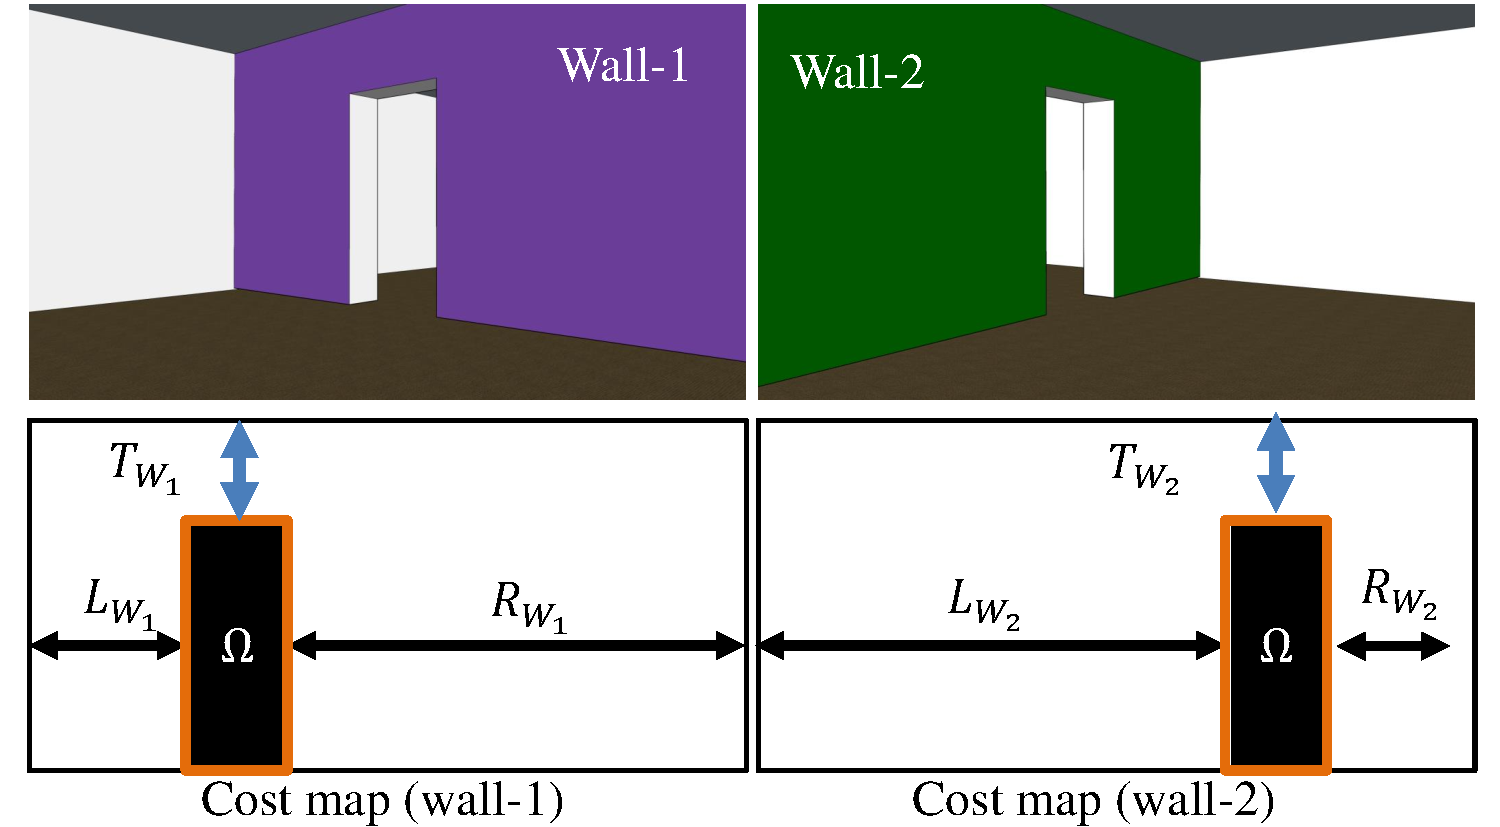
\includegraphics[width=85mm]{../figures/wallprofile.pdf}
	\end{center}
	\vspace{-0.2cm}
	\caption{Once the rectangle $\Omega$ is extracted, we compute
 the left, the right, and the top margins between the rectangle and the
 wall.}
% three distances for each wall independently, between the side of the rectangle and the side of the wall $L_W, R_W$, and the top of the rectangle and the ceiling.}
	\label{fig:wallprofile}
	\vspace{-0.25cm}
\end{figure}
\begin{figure}[!t]
	\begin{center}
         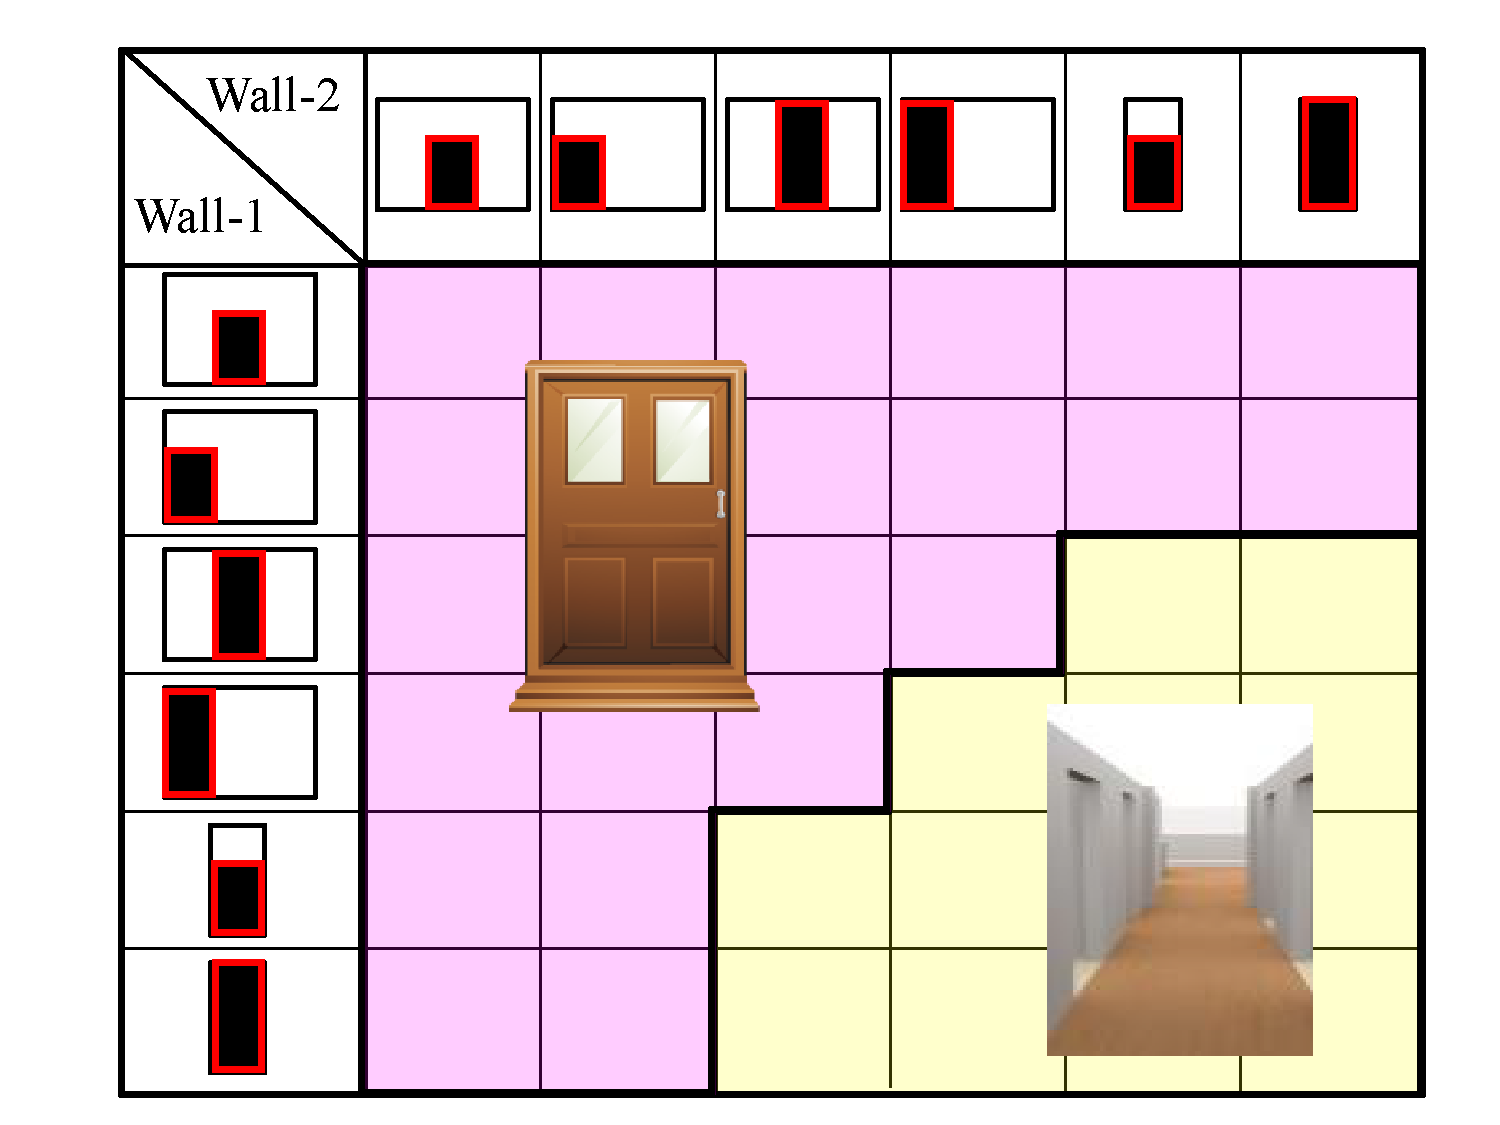
\includegraphics[width=85mm]{../figures/dooranalysis.pdf}
	\end{center}
	\vspace{-0.2cm}
 \caption{Classification table for the room connection types.
 Based on the configuration of the three margins, each wall is
 classified into six types. The combination of the two wall types
 classifies the room connection into either ``door'' (top-left) or
 ``merge'' (bottom-right).
 % Here
 %        we categorize each wall into one of six condition based on the
 %        wing and top distances, and refer the cell that is provided by a
 %        combination of labels of two walls. \yasu{change the icons at
 % the left and the top, which are very confusing.}\yasu{make door and
% open icon better.}}
 } \label{fig:dooranalysis}
	\vspace{-0.25cm}
\end{figure}
This section details in the classification of the room connection, given
the rectangles on the two opposing walls.
%(we should note that $\lambda_1 = 0.01$, and $\lambda_2 = 0.001$ in the
%experiments).
We measure the three margins between the door and the wall boundary in
each wall as in Fig.~\ref{fig:wallprofile}. Depending on the existence
of the margins against some thresholds, each wall is classified into six
different configurations (See Fig.\ref{fig:dooranalysis}). Finally, the
room connection type (either door or merge) is determined as shown in
the table. The thresholds for the horizontal and the vertical margins
are $0.13$m and $0.05 \times \mbox{\{wall height\}}$, respectively.


% Each of the two walls are classified into three types: 

% Then, we assign two types of labels to each wall based on the distances
% mentioned above. The first label is the wing label which has three
% conditions; (w-1) two-side wing: $L_W\geq \alpha_1, R_W \geq \alpha$,
% (w-2) one-side wing: $L_W\geq \alpha_1, R_W < \alpha$ or $R_W\geq
% \alpha_1, L_W < \alpha$, (w-3) $L_W < \alpha_1, R_W < \alpha$. The
% second label is the top label which has two conditions; (t-1) $T_W \geq
% \beta$, (t-2) $T_W < \beta$.

% Using the combination of those two labels (The total combination of
% two-labels are six ($3\times2$)), we refer the classification
% table~\Fref{fig:dooranalysis} to recover the door connection type. Here
% we use $\alpha_1 = 0.13$ m and $\alpha_2 = 0.05\times(WallHeight)$ in
% our experiments.


%
% The classification table evaluates the standard door geometry, where the
% door connection generally has wings and the top, but open connection
% does not have them, however the actually connection is more complex than
% that due to the complex ceiling geometry or noises on the point
% cloud. In those cases, we observed that we often mis-classify the open
% connection as a door. For avoiding mis-classification, we also consider
% the statistics of the dataset. Assuming that the door size of the same
% building are close with each other, we consider the too large door as a
% mis-classified open connection. And if the width of the rectangle is
% larger than min(doorwidth) + std(doorsize(:,1)), we classify as the open
% connection instead of the door connection.


